
\documentclass[a4paper, 12pt]{article}
\usepackage[a4paper,top=1.5cm, bottom=1.5cm, left=1cm, right=1cm]{geometry}
\usepackage{cmap}					
\usepackage{mathtext} 				
\usepackage[T2A]{fontenc}			
\usepackage[utf8]{inputenc}			
\usepackage[english,russian]{babel}
\usepackage{multirow}
\usepackage{graphicx}
\usepackage{wrapfig}
\usepackage{tabularx}
\usepackage{float}
\usepackage{longtable}
\usepackage{hyperref}
\hypersetup{colorlinks=true,urlcolor=blue}
\usepackage[rgb]{xcolor}
\usepackage{amsmath,amsfonts,amssymb,amsthm,mathtools} 
\usepackage{icomma} 
\usepackage{euscript}
\usepackage{mathrsfs}
\usepackage{enumerate}
\usepackage{caption}
\usepackage{enumerate}
\mathtoolsset{showonlyrefs=true}
\usepackage{graphicx}
\usepackage{caption}
\usepackage{subcaption}

\DeclareMathOperator{\sgn}{\mathop{sgn}}
\newcommand*{\hm}[1]{#1\nobreak\discretionary{}
	{\hbox{$\mathsurround=0pt #1$}}{}}

\begin{document}
	\begin{center}
		\textit{Федеральное государственное автономное образовательное\\ учреждение высшего образования }
		
		\vspace{0.5ex}
		
		\textbf{«Московский физико-технический институт\\ (национальный исследовательский университет)»}
	\end{center}
	
	\vspace{10ex}
	
	
	\begin{center}
		\vspace{13ex}
		
		\textbf{Лабораторная работа №1.1.1}
		
		\vspace{1ex}
		
		по курсу общей физики
		
		на тему:
		
		\textbf{\textit{<<Измерение удельного сопротивления нихромовой проволочки>>}}
		
		\vspace{30ex}
		
		\begin{flushright}
			\noindent
			\textit{Работу выполнил:}\\  
			\textit{Никифоров Дмитрий \\(группа Б02-205)}
		\end{flushright}
		\vfill
		Долгопрудный \\ \today
		
	\end{center}
\newpage


\section{Введение}
\textbf{Аннотация:}
\\
В работе измеряется удельное сопротивление тонкой проволоки круглого сечения, изготовленной из нихромового сплава. Геометрические размеры образца измеряются с помощью линейки, штангенциркуля и микрометра. Для измерения сопротивления используются следующие методы: 
\\
-- определение углового коэффициента наклона зависимости напряжения на проволоке от тока через неё, измеряемых с помощью аналоговых и цифровых вольтметров и амперметров, 
\\
-- измерение с помощью моста постоянного тока. 
\\Детально исследуется систематические и случайные погрешности проводимых измерений.
\bigskip\\
\textbf{Цель работы:} измерить удельное сопротивление проволоки и вычислить систематические и случайные погрешности при использовании таких измерительных приборов, как линейка, штангенциркуль, микрометр, амперметр, вольтметр и мост постоянного тока.
\bigskip\\
\textbf{Оборудование:} линейка, штангенциркуль, микрометр, отрезок проволоки из нихрома, амперметр, вольтметр, источник ЭДС, мост постоянного тока, реостат, ключ.

\section{Теоритические сведения}
\begin{center}{Удельное сопротивление проволоки из однородного материала постоянного сечения измеряется по формуле:}
	\begin{equation}\label{r1}
		\rho = R_\text{пр}\cdot\frac{S_\text{пр}}{l} = \frac{R_\text{пр}}{l} \cdot \frac{\pi d^2}{4}
	\end{equation}
\end{center}
В данной работе измерять сопротивление $R_\text{пр}$ предлагается с помощью  схемы представленной на рис.\ref{sexes}

\begin{figure}[h]
	\centering
	\includegraphics[scale=1.5]{"schema111.png"}
	\caption{Схема для измерения сопротивления}
	\label{sexes}
\end{figure}

Пусть $V$ и $I$ -- показания вольтметра и амперметра, при расчете сопротивления только этими данными: $R_\text{пр1} = V_\text{1}/I_\text{1}$ найденное сопротивление будет отличаться от искомого $R_\text{пр}$ из-за внутренних сопротивлений приборов.

\begin{center}{Учитывая сопротивления приборов получаем:}
	\begin{equation}\label{r1}
		R_\text{пр1} = \frac{V_1}{I_1} = R_\text{пр}\frac{R_V}{R_\text{пр} + R_V}
	\end{equation}
\end{center}

\begin{center}
	Эту формулу можно преобразовать в удобную для наc форму:
	\begin{equation}\label{r3}
		R_\text{пр} = \frac{R_\text{пр1}}{1 - \left(\frac{R_\text{пр1}}{R_V} 	\right)} \approx R_\text{пр1}\left(1 + \frac{R_\text{пр1}}{R_V} \right)
	\end{equation}
\end{center}

Таким образом получаем пример систематической ошибки, возникающей из-за упрощения расчетной формулы. Для нашей схемы сопротивление $R_\text{пр}$ оказывается заниженным относительно рассчитанного.

Более точным методом измерения сопротивлений является метод моста постоянного тока (мост Уитстона).

\section{Оборудование и экспериментальные погрешности}

\subsection{Характеристики измерительных приборов}
\begin{longtable}[H]{|c|c|c|}
	\hline
	& Вольтметр & Миллиамперметр\\
	\hline
	Система & Магнитоэлектрическая & Электромагнитная \\
	Класс точности & 0,5 & --- \\
	Предел измерений $x_\text{П}$ & 0,75 В & 2 А\\
	Число делений шкалы $n$ & 150 & ---\\
	Цена делений $x_\text{П}/n$ & 5 мВ/дел & ---\\
	Чувствительность $n/x_\text{П}$ & 200 дел/В & --- \\
	Абсолютная погрешность $\Delta x_\text{М}$ & 6,25 мВ & 0,3 мА -- 2 мА\\
	Внутреннее сопротивление прибора & 5000 Ом & 1,2 Ом \\
	\hline
\end{longtable}
\textbf{Вольтметр:}
\begin{equation}
	 \sigma_\text{V} = \frac{c_V}{2} + \frac{\gamma x_\text{П}}{100} = 6,25\text{ мВ}
\end{equation}

\textbf{Амперметр:} 
\begin{equation}
	 \sigma_\text{I} = 0,005I + 2c_A
\end{equation}

\textbf{Штангенциркуль:} $ \sigma_\text{ш} = 0,05 \text{ мм}$\\

\textbf{Микрометр:} $ \sigma_\text{м} = 0,01 \text{ мм}$
\section{Измерения}
\subsection{Измерение диаметра проволоки}
\begin{table}[h]
	\begin{center}
		\begin{tabular}{|c|c|c|c|c|c|c|c|c|c|c|c|}
			\hline
			№ & 1 & 2 & 3 & 4 & 5 & 6 & 7 & 8 & 9 & 10 & ср. \\
			\hline
			$d_\text{ш}$, мм & 0,3 & 0,3& 0,3& 0,3& 0,3& 0,3& 0,3& 0,3& 0,3& 0,3& 0,3\\ 
			\hline
			$d_\text{м}$, мм & 0,34 & 0,34 & 0,32 & 0,31 & 0,32& 0,31& 0,32& 0,32& 0,32& 0,33& 0,323\\ 
			\hline
		\end{tabular}
	\end{center}
	\caption{Результаты измерения диаметра проволоки}
	\label{dtab}
\end{table}

При измерении штангенциркулем случайная погрешность отсутствует, а значит можно учитывать только системную погрешность: $d_\text{ш} = \left( 0,30 \pm 0,05 \right) \text{ мм}$.

При измерении же микрометром нужно учитывать и системную и случайную погрешость:
$$\sigma_\text{сист}=0,01\text{ мм}\;\;\;\;\;\; \sigma_\text{сл}=\frac{1}{N} \sqrt{\sum_{i=1}^{n}(d_i - \overline{d})^2}=\frac{1}{10} \sqrt{4,3\cdot 10^{-4}}\approx 2\cdot 10^{-3} \text{ мм}$$
$$\sigma_{d_\text{м}} = \sqrt{\sigma_\text{сист}^2+\sigma_\text{сл}^2}\approx 0,01 \text{ мм}$$
\noindent тогда $d_\text{м} = \left( 0,32 \pm 0,01 \right) \text{ мм}$.

Площадь поперечного сечения проволоки можно вычислить зная диаметр, используя диаметр найденный с помощью микрометра мы уменьшим погрешность площади. Вычислим площадь и ее погрешность:

\begin{equation}
	S_\text{пр} = \frac{\pi d_\text{м}^2}{4} = \frac{3,1415\cdot (0,323)^2}{4} \approx 0,1 \text{ мм}^2
\end{equation}

\begin{equation}
	\sigma_S = 2\frac{\sigma_{d_\text{м}}}{d_\text{м}}\cdot S = 2\frac{0,01}{0,323} \cdot 0,1 \approx 6,2\cdot 10^{-3} \text{ мм}^2
\end{equation}

С учетом погрешности получаем, что $S_\text{пр} = \left( 0,1 \pm 6,2 \cdot 10^{-3}\right) \text{ мм}^2$ т.е. площадь поперченого сечения определена с точностью 6,2\%


\subsection{Измерение поправок при измерении сопротивления}

Поправки при измерении $R_\text{пр}$ это дополнительные коэффиценты на которые мы умножаем полученное сопротивление, для учета сопротивления измерительных приборов. Для нашей схемы эта поправка будет равняться $\frac{R_\text{пр1}}{R_V}\cdot 100\% = 0,1\%$.

\subsection{Снятие показаний вольтметра и амперметра, обработка полученных данных}

Ниже представленны данные, снятые с приборов в ходе эксперимента, для проволок разной длины: $l_1=(20,0 \pm 0,1)\text{ см}$; $l_2=(30,0 \pm 0,1) \text{, см}$; $ l_3=(50,0 \pm 0,1)\text{ см}$ :
\begin{longtable}[H]{|c|c|c||c|c|c||c|c|c|}
	\hline
	\multicolumn{3}{|c||}{$l = 20 \text{ см}$} & \multicolumn{3}{c||}{$l = 30 \text{ см}$} & \multicolumn{3}{c|}{$l = 50 \text{ см}$}  \\
	\hline
	V, дел & V, мВ & I, мА & V, дел & V, мВ & I, мА & V, дел & V, мВ & I, мА \\
	\hline
	26 & 130 & 65,64 & 39 & 195 & 64,16 & 61 & 305 & 61,89 \\
	\hline
	36 & 180 & 89,79 & 49 & 245 & 81,84 & 69 & 345 & 70,19 \\
	\hline
	48 & 240 & 119,27 & 57 & 285 & 95,25 & 80 & 400 & 81,67 \\
	\hline
	52 & 260 & 129,00 & 69 & 345 & 114,72 & 88 & 440 & 89,60 \\
	\hline
	58 & 290 & 144,60 & 81 & 405 & 135,84 & 96 & 480 & 98,14 \\
	\hline
	69 & 345 & 172,42 & 96 & 480 & 160,56 & 102 & 510 & 103,50 \\
	\hline
	83 & 415 & 207,68 & 107 & 535 & 178,97 & 111 & 555 & 113,08 \\
	\hline
	91 & 455 & 226,38 & 115 & 575 & 191,30 & 120 & 600 & 122,09 \\
	\hline
	105 & 525 & 261,64 & 123 & 615 & 204,34 & 128 & 640 & 130,25 \\
	\hline
	127 & 635 & 315,85 & 132 & 660 & 220,42 & 134 & 670 & 136,08 \\
	\hline
	138 & 690 & 342,99 & 140 & 700 & 234,00 & 140 & 700 & 142,42 \\
	\hline
	150 & 750 & 371,78 & 147 & 735 & 245,50 & 147 & 735 & 149,15 \\
	\hline
	
	\caption{Снятая зависимость $V(I)$ для проволок разных длин}
\end{longtable}

\newpage

Построим графики по данным из таблицы: рис. \ref{graph}.
\begin{figure}[h!]
	\centering
	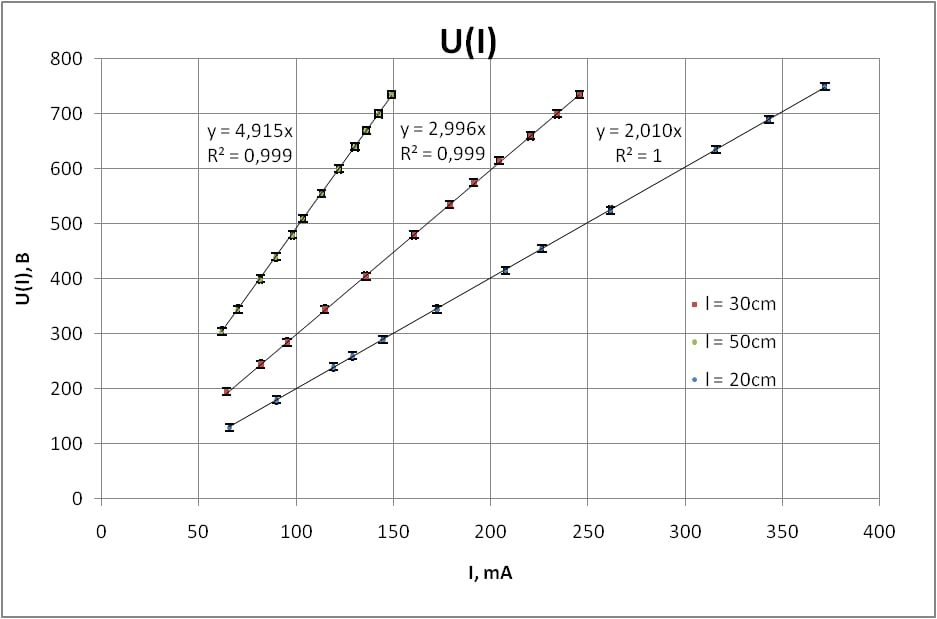
\includegraphics[scale = 0.55]{111_graph}
	\caption{Графики зависимости $V(I)$}
	\label{graph}
\end{figure}

Для каждой длины проволоки $l$ найдем  сопротивление и погрешности методом наименьших квадратов по формулам:

\begin{equation}
	R_\text{ср} = \frac{\langle VI\rangle}{\langle I^2 \rangle}
\end{equation}


\begin{minipage}{0.45\textwidth}
	\centering
	\begin{equation}
		\sigma_{R_\text{ср}}^{\text{случ}} = \frac{1}{\sqrt{12}}\sqrt{\frac{\langle V^2 \rangle}{\langle I^2 \rangle} - R_\text{ср}^2}
	\end{equation}
\end{minipage}
\begin{minipage}{0.45\textwidth}
	\centering
	
	\begin{equation}
		\sigma_{R_\text{ср}}^{\text{сист}} = R_\text{ср}\sqrt{\left(\frac{\sigma_V}{V} \right)^2 + \left(\frac{\sigma_I}{I} \right)^2}
	\end{equation}
\end{minipage}

\begin{equation}
	\sigma_{R_\text{ср}} = \sqrt{\sigma_{\text{сист}}^2 + \sigma_{\text{случ}}^2}
\end{equation}

\noindent где $V$ и $I$ -- максимальные значения тока и напряжений, $\sigma_V = 6,25 \text{ мВ}$, а $\sigma_I = 2 \text{ мА}$. Рассчитываем сопротивление с учетом поправки для схемы и погрешности:

\begin{longtable}[H]{|c||c||c|}
	\hline
	$l = 20 \text{ см}$ & $l = 30 \text{ см}$ & $l = 50 \text{ см}$ \\
	\hline
	$R_\text{ср} = 2,010\text{ Ом}$ & $R_\text{ср} = 2,996 \text{ Ом}$ & $R_\text{ср} = 4,915 \text{ Ом}$ \\
	\hline
	$R_\text{пр} = 2,012 \text{ Ом}$ & $R_\text{пр} = 2,999 \text{ Ом}$ & $R_\text{пр} = 4,920 \text{ Ом}$\\
	\hline
	$\sigma_R^\text{случ} = 0,002\text{ Ом}$ & $\sigma_R^\text{случ} = 0,003\text{ Ом}$ & $\sigma_R^\text{случ} = 0,003\text{ Ом}$ \\
	\hline
	$\sigma_R^\text{сист} = 0,020 \text{ Ом}$ & $\sigma_R^\text{сист} = 0,030 \text{ Ом}$ & $\sigma_R^\text{сист} = 0,048 \text{ Ом}$ \\
	\hline
	$\sigma_{R_\text{ср}} = 0,020 \text{ Ом}$ & $\sigma_{R_\text{ср}} = 0,030 \text{ Ом}$ & $\sigma_{R_\text{ср}} = 0,048 \text{ Ом}$ \\
	\hline
	
	\caption{Экспериментально полученные сопротивления и погрешности}
	\label{R}
\end{longtable}

\subsection{Нахождение сопротивления с помощью моста}

\begin{longtable}[H]{|c|c|c|c|}
	\hline
	l, см & 20 & 30 & 50 \\
	\hline
	$R_\text{пр} \text{, Ом}$ & 2,0408 & 3,0546 & 5,0416 \\
	\hline
	
	\caption{Сопротивления, полученные с помощью моста}
	\label{most}
\end{longtable}

Сравниваем результаты полученные косвенно с результатами на мосте. Результаты измерений первых двух длин попадают в предел $\pm2\sigma_R$ из таб.\ref{R}. Измерение 3 попадает в предел $\pm3\sigma_R$.

\newpage

\subsection{Вычисление удельного сопроивления проволоки}

Удельное сопротивление проволоки изготовленной из однородного материала и погрешность могут быть определены по формулам:

\begin{minipage}{0.45\textwidth}
	\centering
	\begin{equation}
		\rho = R_\text{пр}\cdot\frac{S_\text{пр}}{l} = \frac{R_\text{пр}}{l} \cdot \frac{\pi d^2}{4}
	\end{equation}
\end{minipage}
\begin{minipage}{0.45\textwidth}
	\centering
	\begin{equation}
		\sigma_\rho = \rho\sqrt{\left(\frac{\sigma_R}{R}\right)^2 + \left( 2\frac{\sigma_d}{d} \right)^2 + \left( \frac{\sigma_l}{l}\right)^2}
	\end{equation}
	
\end{minipage}

\bigskip
\noindent где $R_\text{пр}$ -- сопротивление измеряемого отрезка проволоки, $S_\text{пр}$ -- площадь поперечного сечения проволоки, $l$ -- его длина, а $d$ -- диаметр проволоки.

Занесем полученные результаты в таблицу
\begin{longtable}[H]{|c||c||c|}
	\hline
	$l \text{, см}$ & $\rho$, $ 10^{-6} \text{ Ом} \cdot \text{мм}^2 /\text{м}$ & $\sigma_\rho$, $ 10^{-6} \text{ Ом} \cdot \text{мм}^2 / \text{м}$\\
	\hline
	20 & 0,84 & 0,05\\
	\hline
	30 & 0,83 & 0,05\\
	\hline
	50 & 0,83 & 0,05\\
	\hline
	\caption{Удельные сопротивления участков проволоки различной длины}
\end{longtable}

Конечным значением удельного сопротивления лучше считать удельное сопротивления участка проволоки длиной 50 см, так как его сопротивление наибольшее, что означает наименьшую погрешность и наибольшую точность измерения. В таком случае: $\rho = \left( 0,83 \pm 0,05 \right) \cdot 10^{-6} \text{ Ом}\cdot \text{мм}^2/\text{м}$.

\subsection{Вывод}
Основной вклад в общую ошибку вносит погрешность измерения площади сечения проволоки(6\%), т.е. точности микрометра не хватает для данного эксперимента.
Допустимые значения удельного сопротивления нихрома: $\rho_\text{таб} = (0,97 - 1,14) \cdot 10^{-6} \text{ Ом}\cdot \text{мм}^2/\text{м}$ 	

Все полученные значения отличаются от табличных на $3\sigma_\rho$. Это можно объяснить тем, что в эксперименте не было учтенно сопротивление проводов; также причиной такого несовпадения результатов с табличными данными может быть различие исследуемых проволочек.




\end{document}